%%%%%%%%%%%%%%%%%%%%%%%%%%%%%
% Standard header for working papers
%
% WPHeader.tex
%
%%%%%%%%%%%%%%%%%%%%%%%%%%%%%

\documentclass[11pt]{article}



%%%%%%%%%%%%%%%%%%%%%%%%%%
%% TEMPLATES
%%%%%%%%%%%%%%%%%%%%%%%%%%


% Simple Tabular

%\begin{tabular}{ |c|c|c| } 
% \hline
% cell1 & cell2 & cell3 \\ 
% cell4 & cell5 & cell6 \\ 
% cell7 & cell8 & cell9 \\ 
% \hline
%\end{tabular}





%%%%%%%%%%%%%%%%%%%%%%%%%%
%% Packages
%%%%%%%%%%%%%%%%%%%%%%%%%%



% encoding 
\usepackage[utf8]{inputenc}
\usepackage[T1]{fontenc}


% general packages without options
\usepackage{amsmath,amssymb,amsthm,bbm}

% graphics
\usepackage{graphicx,transparent,eso-pic}

% text formatting
\usepackage[document]{ragged2e}
\usepackage{pagecolor,color}
%\usepackage{ulem}
\usepackage{soul}


% conditions
\usepackage{ifthen}


\usepackage{natbib}


%%%%%%%%%%%%%%%%%%%%%%%%%%
%% Maths environment
%%%%%%%%%%%%%%%%%%%%%%%%%%

%\newtheorem{theorem}{Theorem}[section]
%\newtheorem{lemma}[theorem]{Lemma}
%\newtheorem{proposition}[theorem]{Proposition}
%\newtheorem{corollary}[theorem]{Corollary}

%\newenvironment{proof}[1][Proof]{\begin{trivlist}
%\item[\hskip \labelsep {\bfseries #1}]}{\end{trivlist}}
%\newenvironment{definition}[1][Definition]{\begin{trivlist}
%\item[\hskip \labelsep {\bfseries #1}]}{\end{trivlist}}
%\newenvironment{example}[1][Example]{\begin{trivlist}
%\item[\hskip \labelsep {\bfseries #1}]}{\end{trivlist}}
%\newenvironment{remark}[1][Remark]{\begin{trivlist}
%\item[\hskip \labelsep {\bfseries #1}]}{\end{trivlist}}

%\newcommand{\qed}{\nobreak \ifvmode \relax \else
%      \ifdim\lastskip<1.5em \hskip-\lastskip
%      \hskip1.5em plus0em minus0.5em \fi \nobreak
%      \vrule height0.75em width0.5em depth0.25em\fi}



%% Commands

\newcommand{\noun}[1]{\textsc{#1}}


%% Math

% Operators
\DeclareMathOperator{\Cov}{Cov}
\DeclareMathOperator{\Var}{Var}
\DeclareMathOperator{\E}{\mathbb{E}}
\DeclareMathOperator{\Proba}{\mathbb{P}}

\newcommand{\Covb}[2]{\ensuremath{\Cov\!\left[#1,#2\right]}}
\newcommand{\Eb}[1]{\ensuremath{\E\!\left[#1\right]}}
\newcommand{\Pb}[1]{\ensuremath{\Proba\!\left[#1\right]}}
\newcommand{\Varb}[1]{\ensuremath{\Var\!\left[#1\right]}}

% norm
\newcommand{\norm}[1]{\left\lVert #1 \right\rVert}



% argmin
\DeclareMathOperator*{\argmin}{\arg\!\min}


% amsthm environments
\newtheorem{definition}{Definition}
\newtheorem{proposition}{Proposition}
\newtheorem{assumption}{Assumption}

%% graphics

% renew graphics command for relative path providment only ?
%\renewcommand{\includegraphics[]{}}


\usepackage{url}





% geometry
\usepackage[margin=2cm]{geometry}



% changes

\usepackage{soul}
\soulregister\cite7
\soulregister\citep7
\soulregister\ref7

\usepackage[final]{changes}
%\usepackage{changes}


\setaddedmarkup{\textcolor{black}{\hl{#1}}}
\setdeletedmarkup{\textcolor{red}{\sout{#1}}}



\usepackage{CJKutf8}
%\begin{CJK*}{UTF8}{zhsong}
%文章内容。
%\clearpage\end{CJK*}
\newcommand{\cn}[1]{
  \begin{CJK*}{UTF8}{gbsn}
  #1
  \end{CJK*}
}



% layout : use fancyhdr package
%\usepackage{fancyhdr}
%\pagestyle{fancy}
%
%\makeatletter
%
%\renewcommand{\headrulewidth}{0.4pt}
%\renewcommand{\footrulewidth}{0.4pt}
%\fancyhead[RO,RE]{}
%\fancyhead[LO,LE]{Models for the co-evolution of cities and networks}
%\fancyfoot[RO,RE] {\thepage}
%\fancyfoot[LO,LE] {}
%\fancyfoot[CO,CE] {}
%
%\makeatother
%

%%%%%%%%%%%%%%%%%%%%%
%% Begin doc
%%%%%%%%%%%%%%%%%%%%%

\begin{document}







\title{Evolving accessibility landscapes: mutations of public transportation networks in China}
\author{\noun{Juste Raimbault}$^{1,2}$\\
$^1$ UPS CNRS 3611 ISC-PIF\\
$^2$ UMR CNRS 8504 G{\'e}ographie-cit{\'e}s
}
\date{}


\maketitle

\justify


\begin{abstract}
Recent years have witnessed an exceptional extension of public transportation networks in People's Republic of China, both at a national scale with the construction of the first HSR railway network of the world, and at local scales with numerous cities developing high coverage subway networks often from scratch. This chapter studies these mutations, both from a qualitative perspective with fieldwork observations and from a quantitative perspective with the study of the evolution of population accessibility landscapes, at a national level and for several cities. We confirm that rebalancing planning objectives are well achieved in terms of accessibility at both scales, when all planned lines will be achieved but already in a significant manner. We finally hypothesize possible paths for the coupled network-territory systems, given the extent without precedent of such mutations.
\end{abstract}

\textbf{Keywords : }\textit{}



%%%%%%%%%%%%%%%%%%%%
\section{Introduction}

This chapter proposes to illustrate the issue of interactions between transportation networks and territories, and more particularly their complexity and the diversity of possible situations already perceptible in a qualitative way (and also subjective in a second time) at the microscopic scale, through concrete fieldwork examples. The geographical subject is Pearl River Delta, in Guangdong province, that we already described before, and more particularly mostly the city of Zhuhai. The objective is to enrich our repertory with concrete situations, to understand if these can be associated to the generic processes we have already exhibited, or if others can be observed at the scales of observation.



%%%%%%%%%%%%%%%%%%%%
\section{Fieldwork observations}


We assume the term of \emph{Geographical Fieldwork}, with all knowledge of epistemological debates its use can raise. Indeed, we extract observations from places that were experimented, in the context of a given problematic~\cite{retaille2010terrain}. Our approach will also highlight the role of representations, underlined as a type of fieldwork in itself by~\cite{lefort2012terrain}, when we will give a subjective view.

In the frame of the European project Medium which establishes a partnership between European and Chinese universities. The project is entitled ``\textit{New pathways for sustainable urban development in China’s medium-sized cities}''. It aims at studying sustainability through an interdisciplinary and multidimensional viewpoint, in the case of rapidly growing urban areas, by concentrating on Chinese medium-sized cities. Three medium-sized Chinese cities were chosen as a case study. The definition of medium-sized cities considered for the project is broader than the official statistical definition of the Chinese government, and covers cities from 1 to 10 millions of inhabitants. More information is available on the website of the project at \url{http://mediumcities-china.org/}. In this context, Zhuhai was chosen as a case study. When the source is not explicitly given, observations come from fieldwork, for which narrative reports are available at % TODO github repo for narrative reports.
 Appendix\ref{app:sec:qualitative}.

 The format of narrative reports is ``on-the-fly'' following the recommendations of \cite{goffman1989fieldwork} for taking notes in an immersive fieldwork in particular, whereas the voluntary subjective position rejoins \cite{ball1990self} which recalls the importance of reflexivity in order to draw rigorous conclusions from qualitative fieldwork observations of which the researcher is a part in itself. The consideration of the researcher as a \emph{subject} in relation with its object of study does not imply in our case a feedback of the researcher on the system because of its size in the case of a transportation network at the scale of the city, and indeed a conditioning of observations by a subjectivity of which we must detach in the posterior exploitation of the observation material, but which ignoring can only increase the biases.


\subsection{Development of a transportation network}

The objective of fieldwork is thus to observe the multiple facets and layers of a complex public transport system which is always transforming, its links with observable urban operations, and to what extent these witness of interaction processes between networks and territories. The spatial extent of observations spans on Zhuhai as an illustration of local transportation but also punctually on other regions in China. These observations have their proper logic in comparison to the modeling of transportation networks or data analysis, such as accessibility studies or interaction models between land-use and transportation, that will be done in the following. Indeed, these fail generally in capturing aspects at a large scale, which are often directly linked to the user, and which can become crucial regarding the effective use of the network. For example, multi-modality is profoundly transformed by the use of the network. Multi-modality consists in the combination of different transportation modes: road, train, metropolitan, tramway, bus, peaceful modes, etc., in a mobility pattern. A multimodal transportation system consists in the superposition of modal layers, and these can be more or less well articulated for the production of optimal routes following multiple objectives (cost, time, generalized cost, comfort, etc.) which themselves depend on the user, and of the mobility pattern. It can in practice made efficient through the emergence of self-organized informal transportation modes, or the establishment of new modes such as bike-sharing, what solves the ``last-mile problem''~\cite{liu2012solving}, which seems to be often neglected in the planning of newly developed areas in China. On the contrary, practical details such as tickets reservation or check-in delays at boarding can considerably influence use patterns.

% NOTE (trad) : here could have cited Lea Wester !

Several trips on the Chinese territory were made to observe the concrete manifestations of the high speed network development. Since 2008, China has established the larger HSR network in the world from scratch, which has a great success and which lines are currently saturated. It answers primary demand patterns in terms of city size, showing that it was planned such that the network answers to territorial dynamics. Its high usage shows the impact of network on mobility, what is a possible precursor of territorial mutations.

To show to what extent territories can influence the development of network in diverse ways, we can take a particular example, linked to the development of tourism, which corresponds to a particular dimension taken into account in planning. Thus, the line between Guangzhou and Guiyang (North-West axis which is precursor of the future direct link Guangzhou-Chengdu) have witnessed the opening of stations specifically for the development of tourism, such as Yangshuo in Guangxi, which number of visits has then strongly increased (see maps in Appendix~\ref{app:sec:qualitative}). One year after the opening of the station, the main road link with the city is still under construction, showing that the different networks react differently to constraints at different levels. A higher number of trains stops on week-ends - more than one each hour, are are full more than two weeks in advance. New mobility patterns can be induced by this new offer, as illustrate the interview of an inhabitant of Guangzhou done in Yangshuo, which came for a short week-end with her colleagues, in the context of a ``team-building'' trip financed by her startup in information technology. These new mobility practices are shown in a second interview of an inhabitant of Beijing met at Emeishan, sent by her company in Industrial Design for a short stay in Chengdu for a training in a local subsidiary. The company prefers the high speed train, and it recently increased the mobility practices for its employees.

A similar strategy can be observed concerning the connection of touristic destinations for the line Chengdu-Emeishan. The principal objective of this line is for now to serve the highly frequented touristic destinations of Emeishan and Leshan. However, the missing link between Leshan and Guiyang is already well advanced in its construction and will complete the direct link between Guangzhou and Chengdu. This reveals diachronic and complementary dynamics of network development following properties of territories. This line is a part of the structuring skeleton of the ``8+8'' recently reformulated by the central government, which corresponds to the general plan for future high speed lines, recently actualized to include 8 North-South parallels and 8 East-West others, completing the 4+4 already realized.  The traversed territories expect a lot from it as shows \cite{lu2012chengdu} for the city of Yibin halfway between Chengdu and Guiyang.

We also observe join mutations of the railway network and of the city. We illustrate thus in Fig.~\ref{fig:qualitative:hsr} the insertion of the HSR in its territories. Direct effects of the network are linked to the development of totally new districts in the neighborhood of new stations, sometimes in an approach of type ``\emph{Transit Oriented Development}'' (TOD)\footnote{As we defined in~\ref{sec:networkterritories}, this planning paradigm aims at articulating the development of an heavy transportation infrastructure with urbanization, typically through a densification around stations.} - we will come back to it with more details. Furthermore, more subtle indirect effects are suggested by clues such as the promotion of operations through advertisement. It shows the socio-economic expectations regarding the network and the local agents which have to contribute to its success: advertisements claiming the merits of high speed, and the selling of appartements in the associated real estate operations. This dynamic seems to contribute to the construction of a ``middle class'' and of the role it has to play in the dynamism of territories~\cite{rocca2008power}\footnote{Construction which is, as \noun{Jean-Louis Rocca} emphasizes, as much concrete since it depends on objective realities, as imaginary in the academic and political discourse, which construct the object simultaneously to its study or use.}. The insertion of lines in territories seems in some case to be forced, as shows the Yangshuo station which exploits the tourism opportunity offered by the passage of the line in a low populated area but which is very attractive by its landscapes, or the new real estate operations in Zhuhai which are not very accessible because of their price.


%%%%%%%%%%%%%
\begin{figure}
	%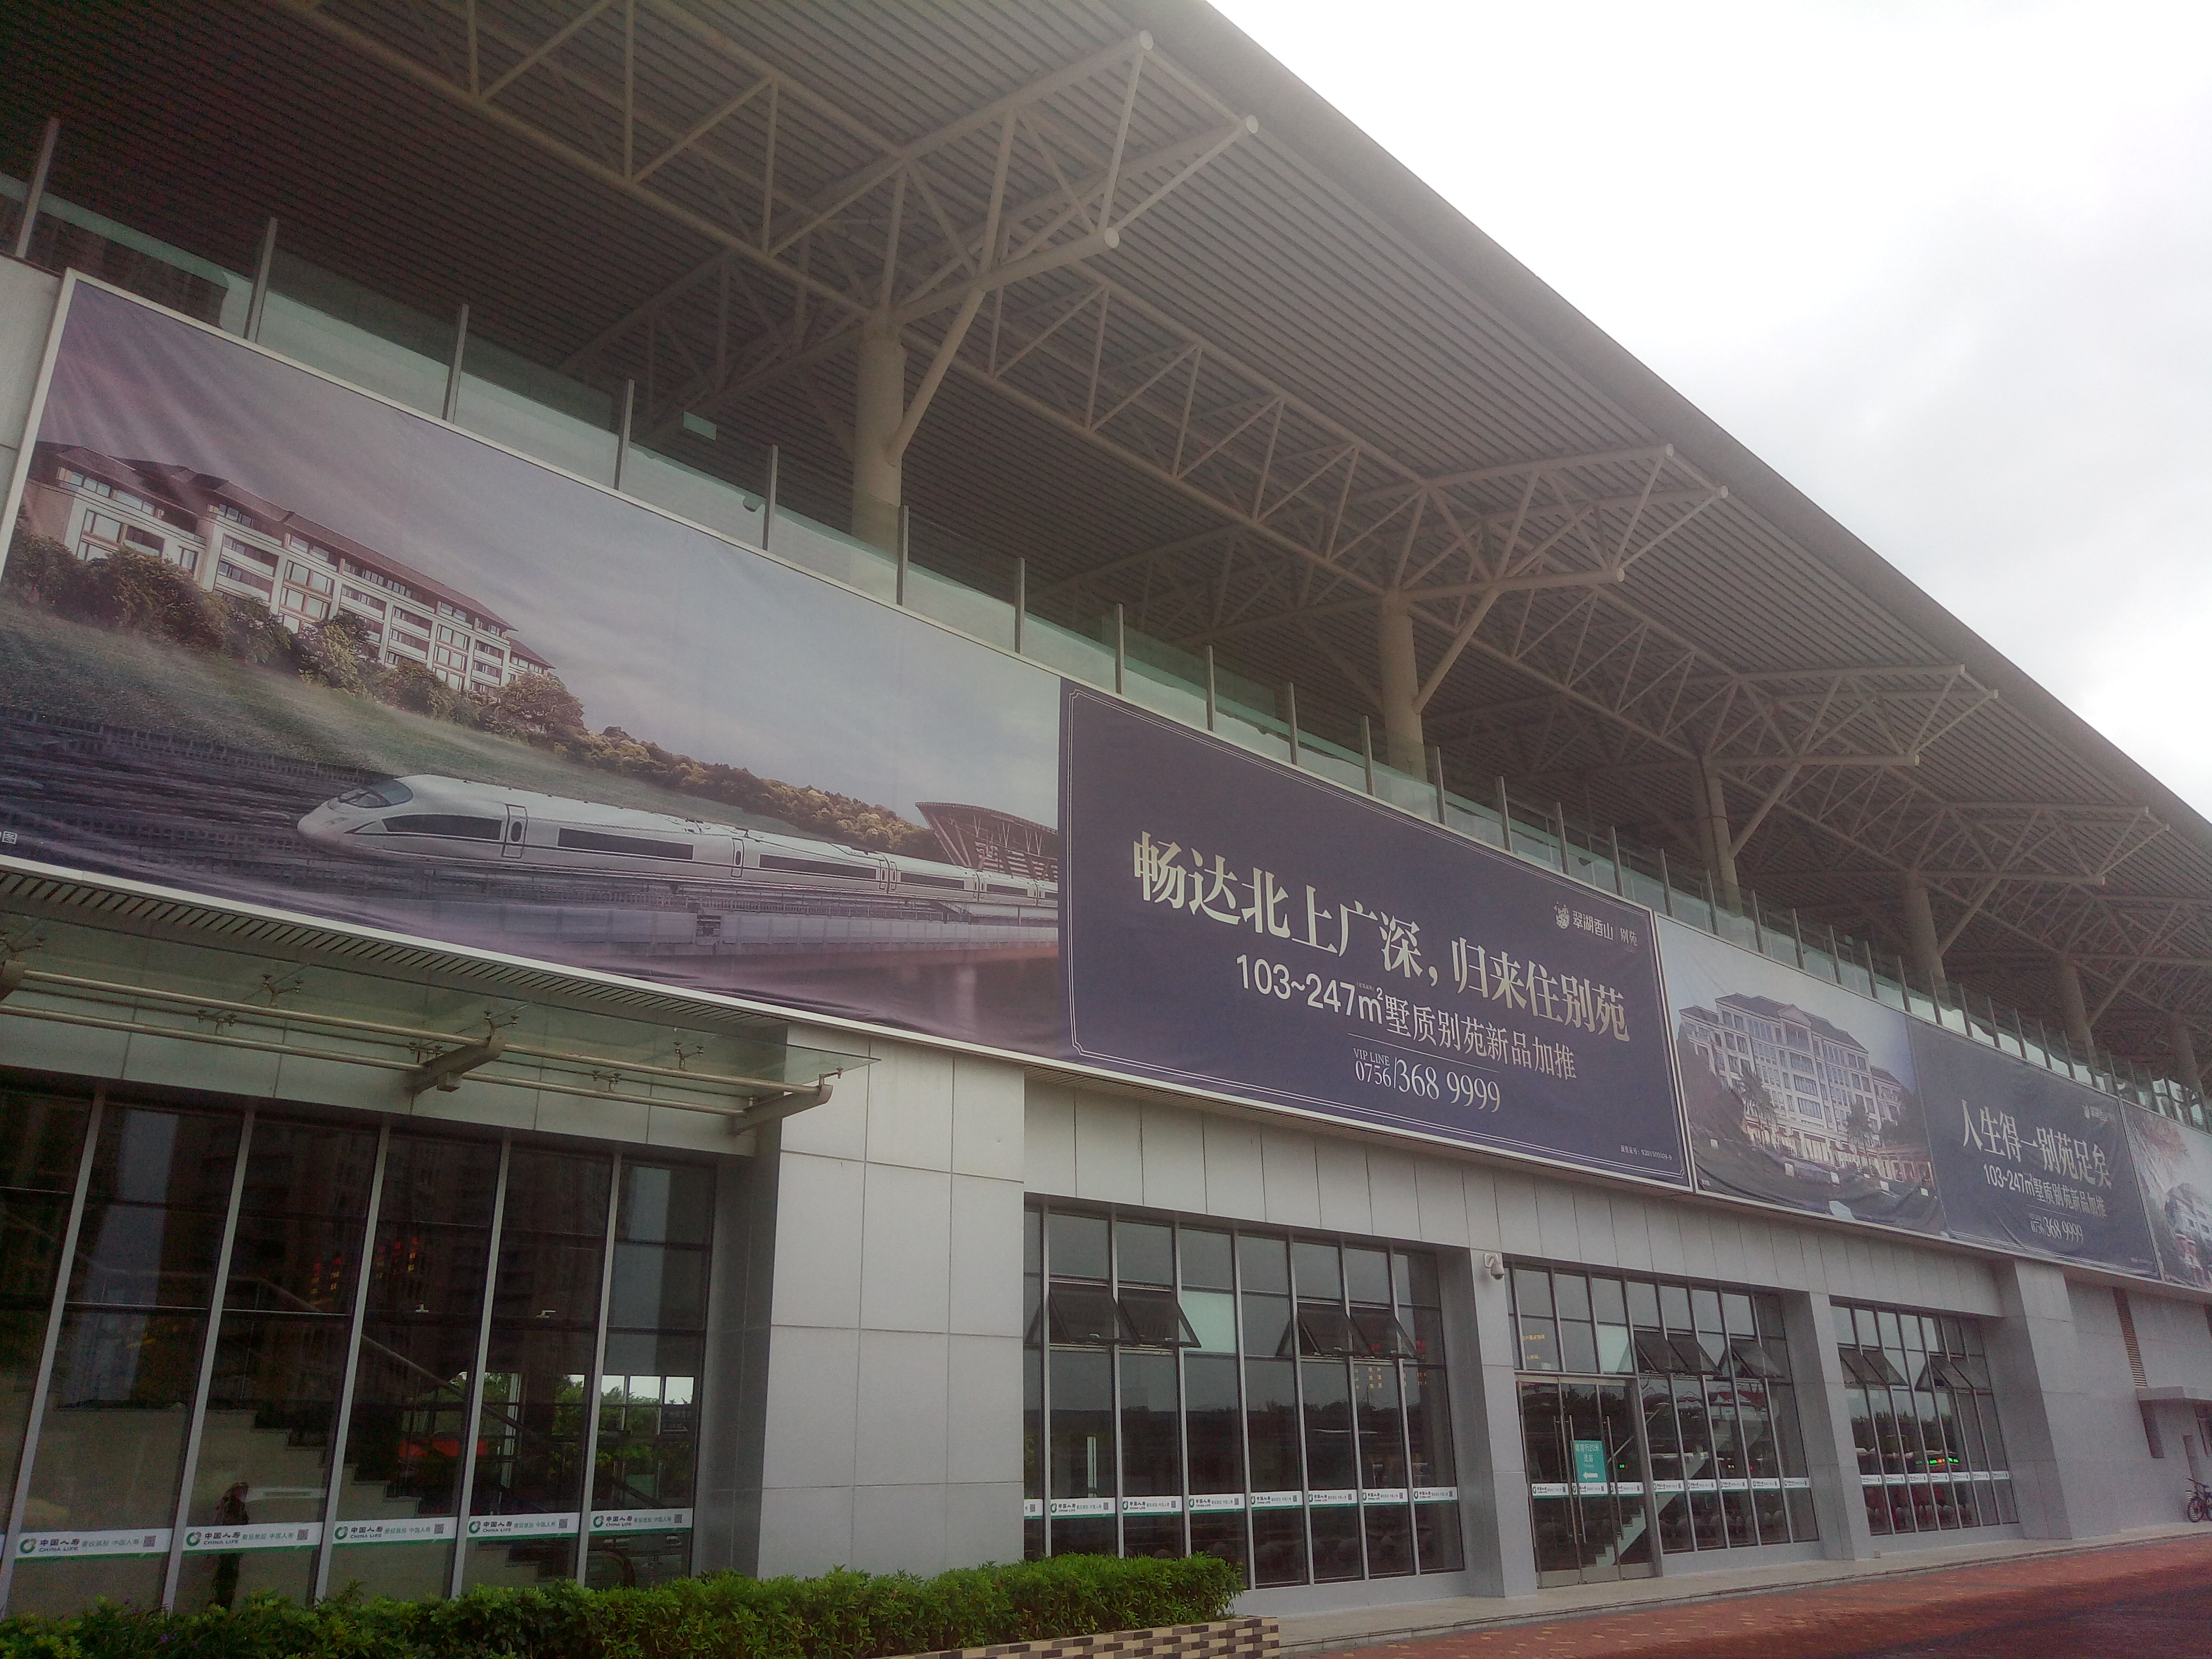
\includegraphics[width=0.48\linewidth]{Figures/Qualitative/tangjia}
	%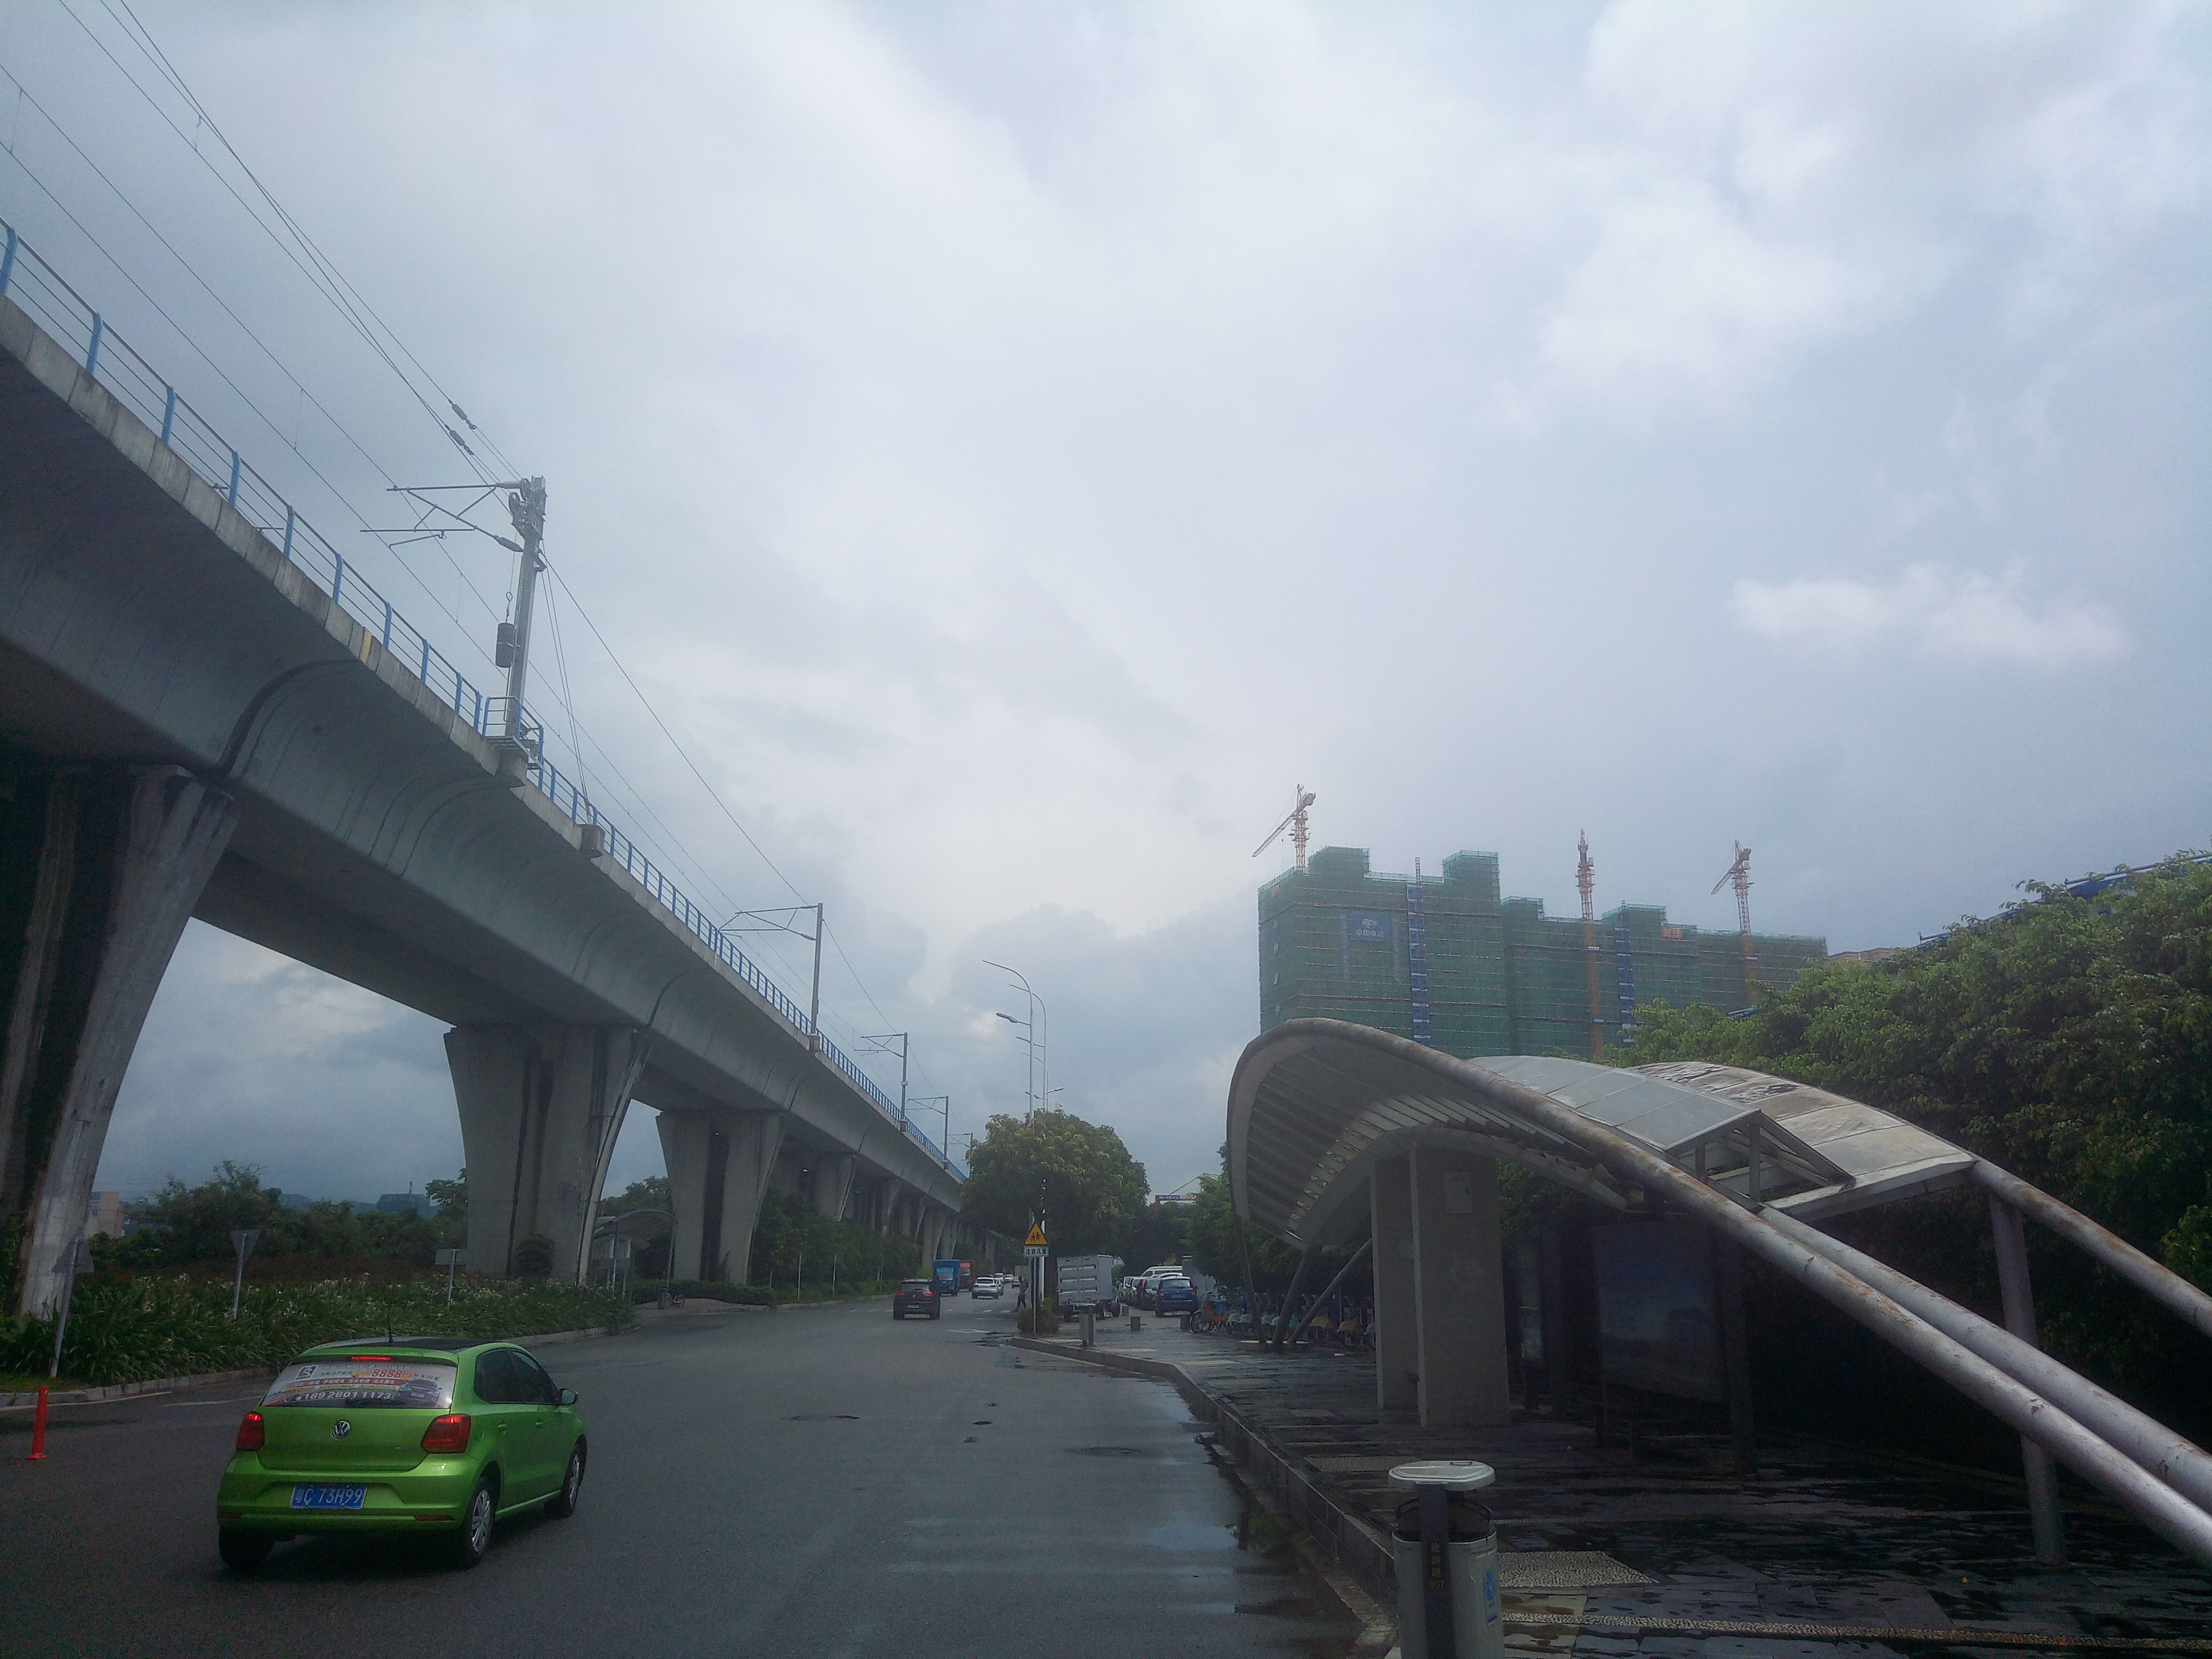
\includegraphics[width=0.48\linewidth]{Figures/Qualitative/zhuhai}\\
	%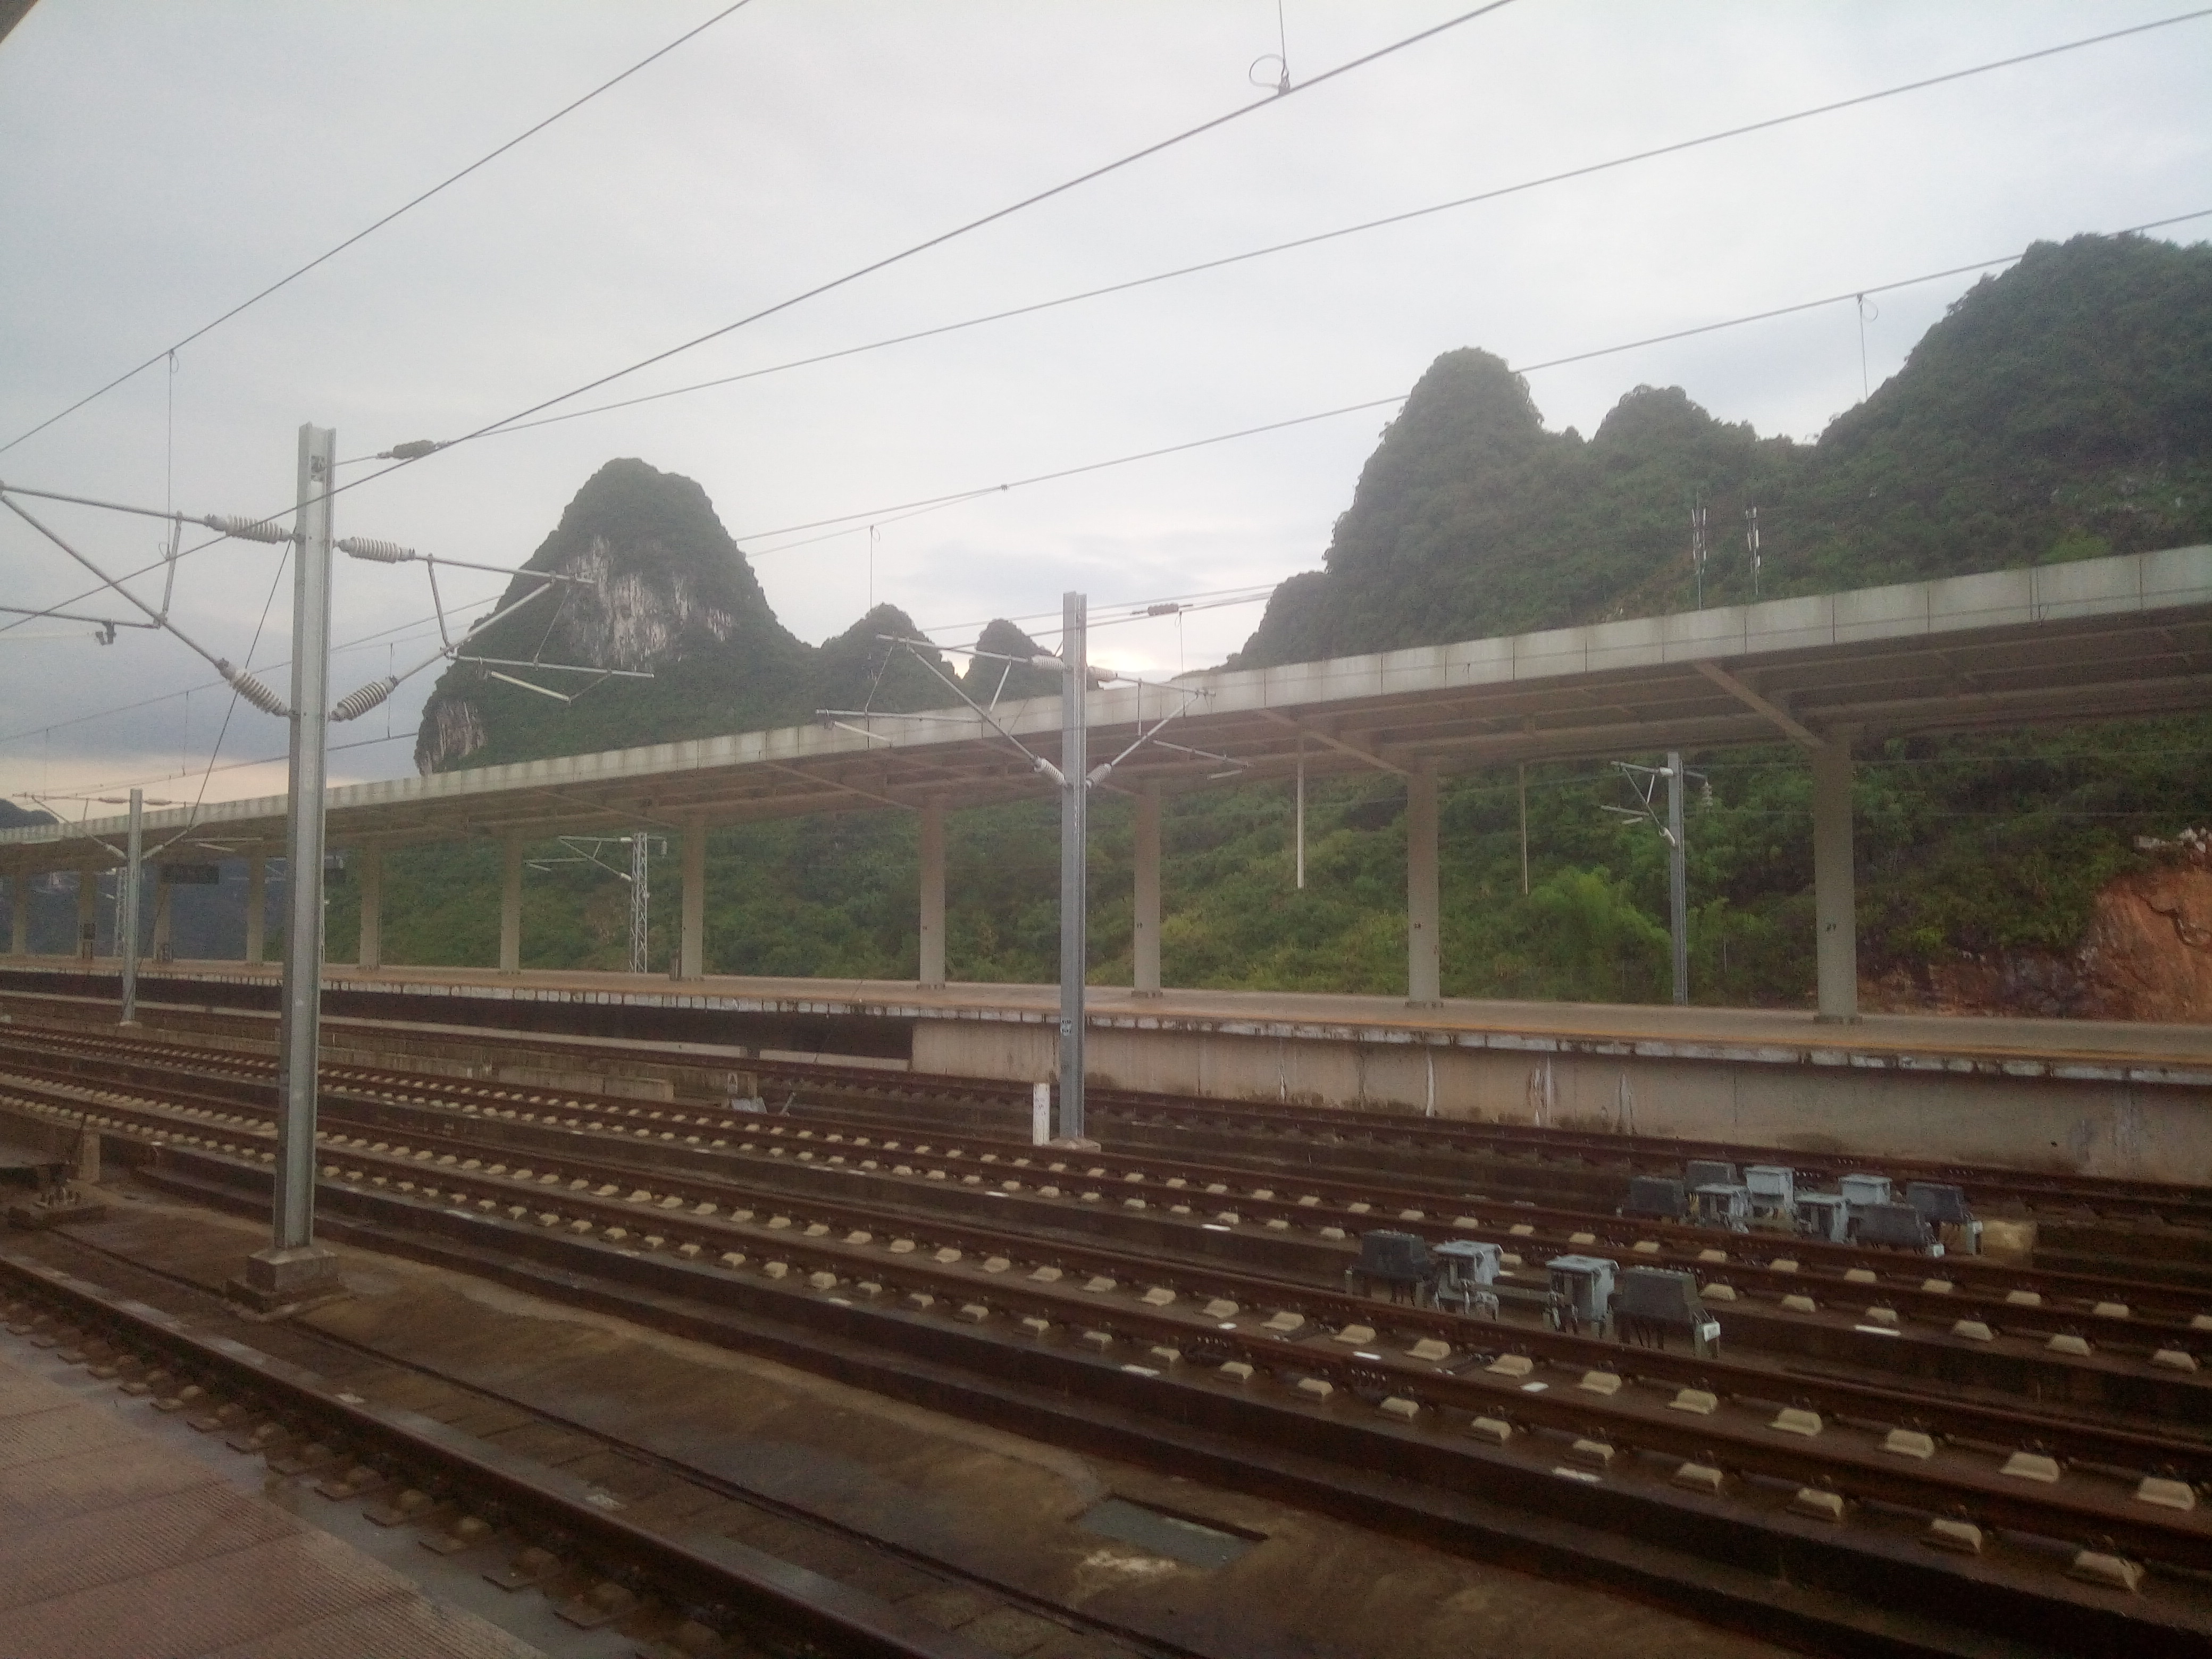
\includegraphics[width=0.48\linewidth]{Figures/Qualitative/yangshuo}
	%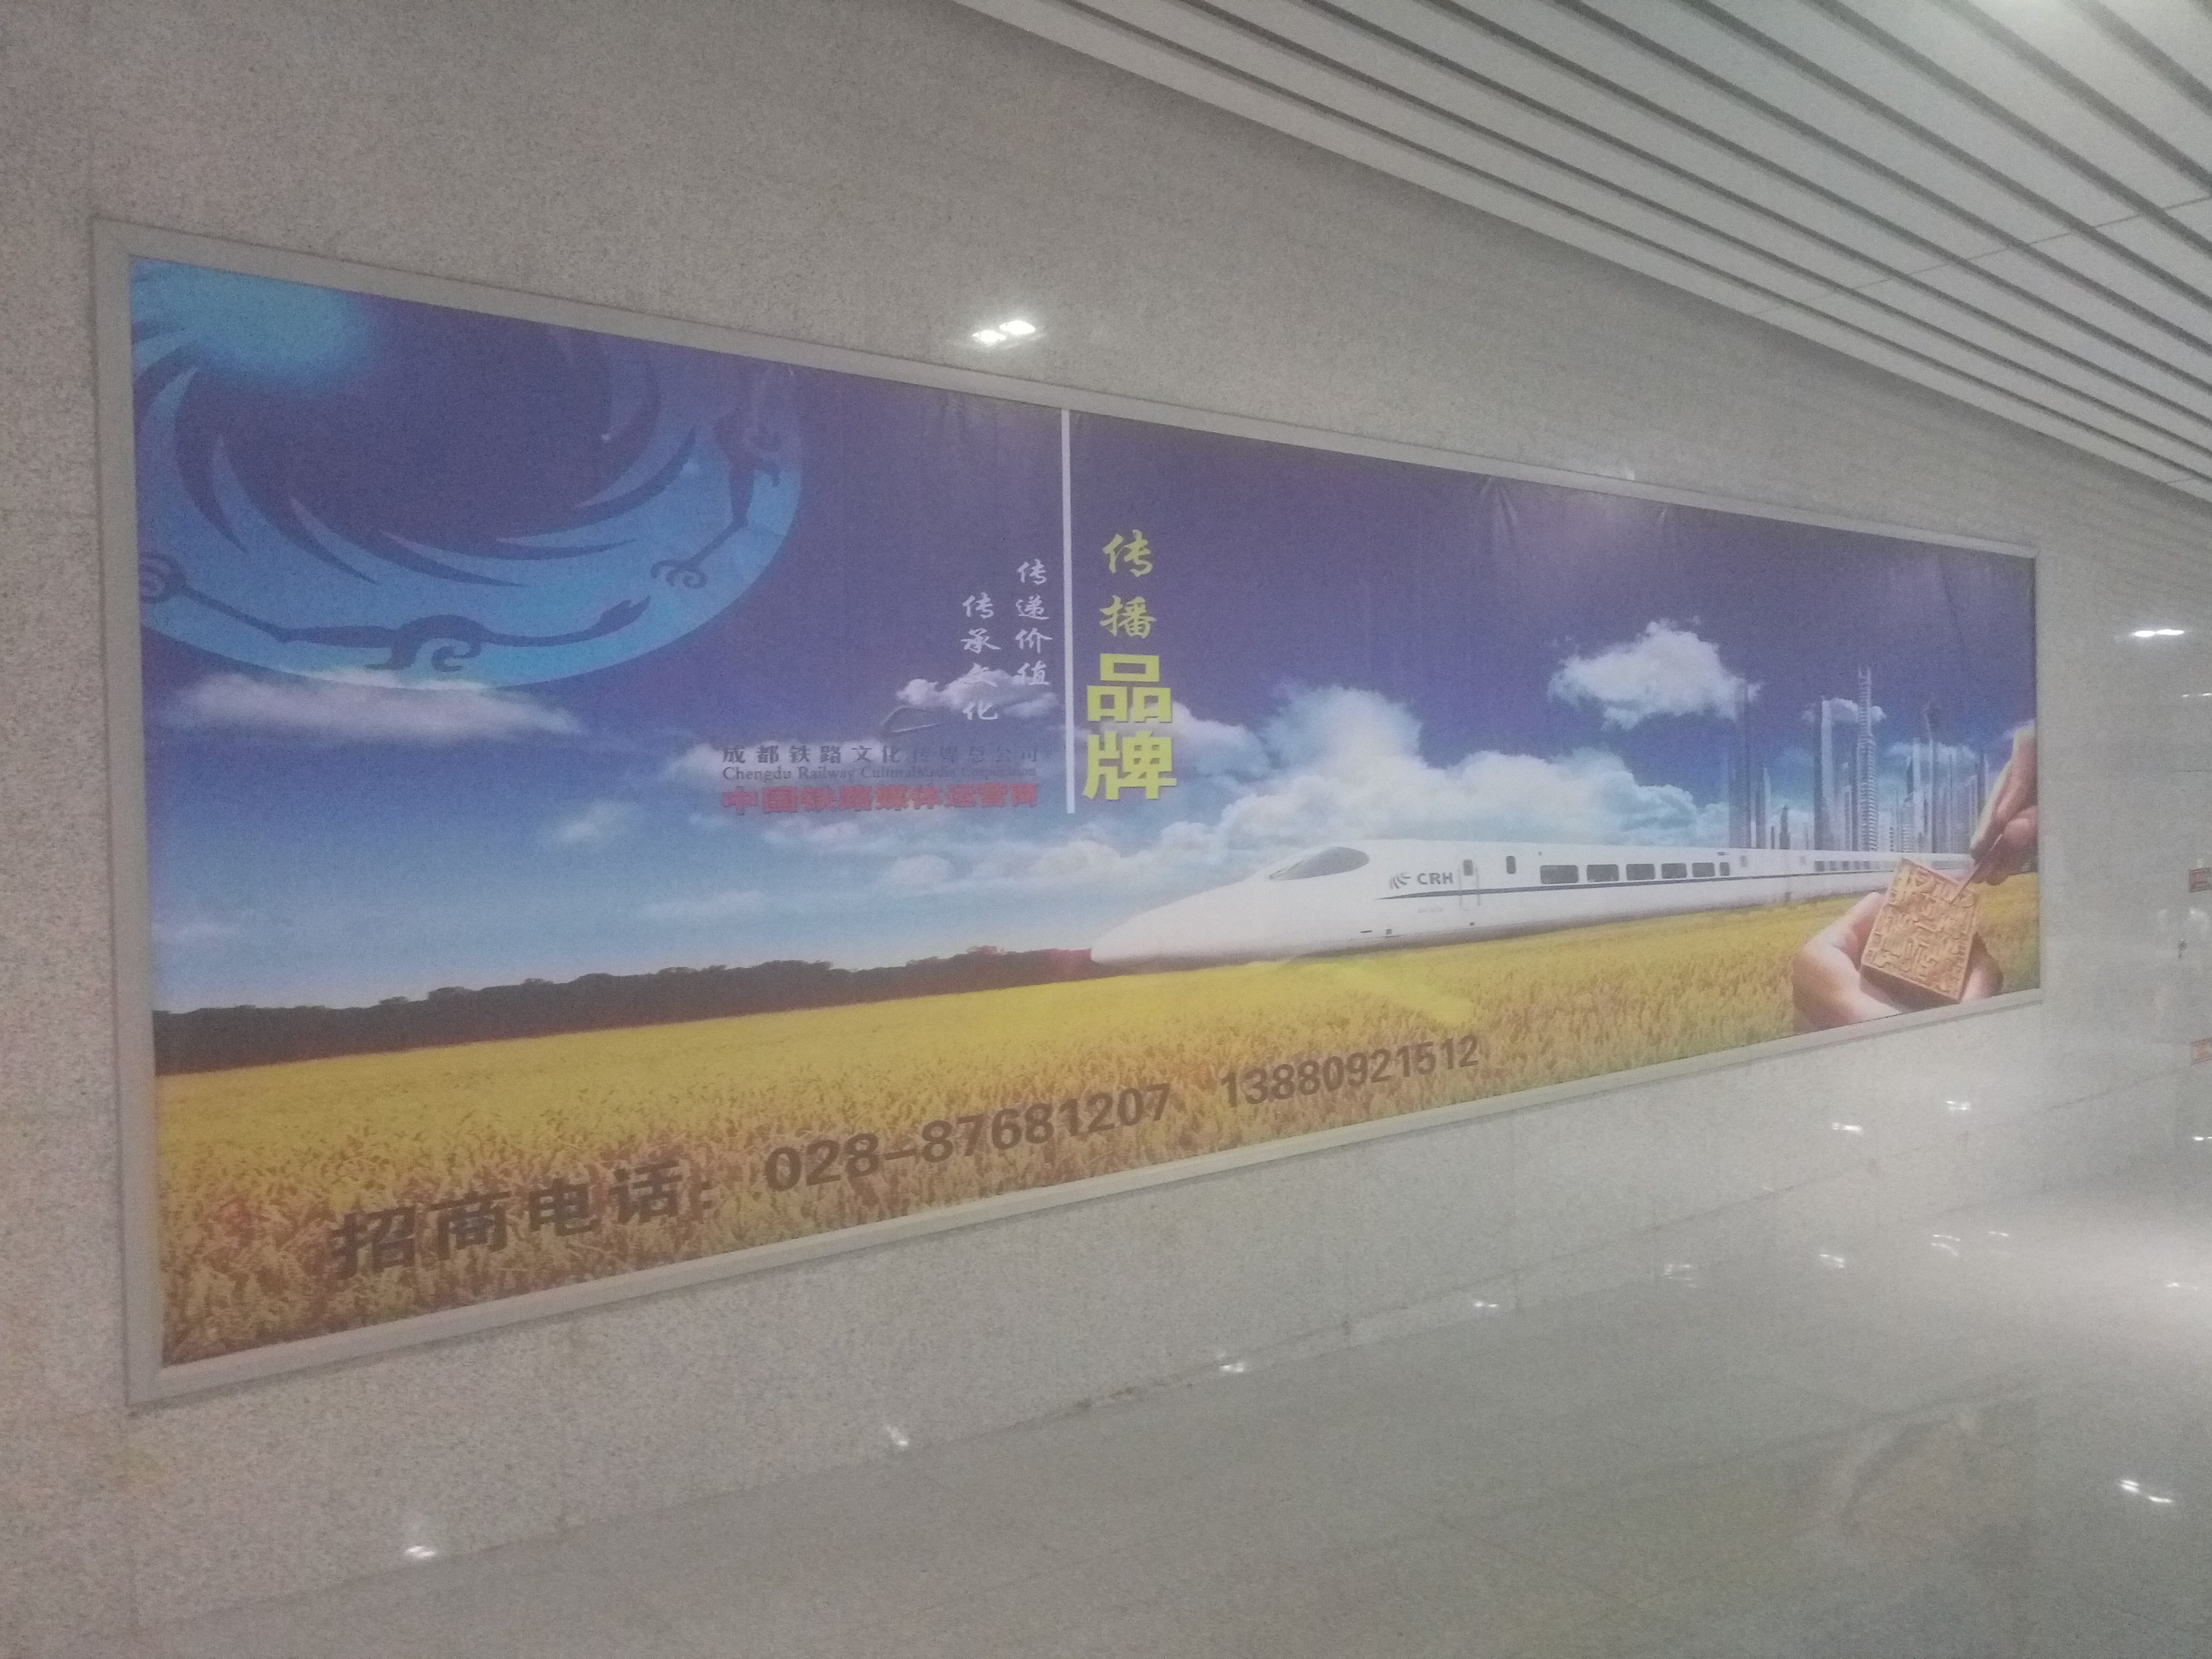
\includegraphics[width=0.48\linewidth]{Figures/Qualitative/chengdu}
	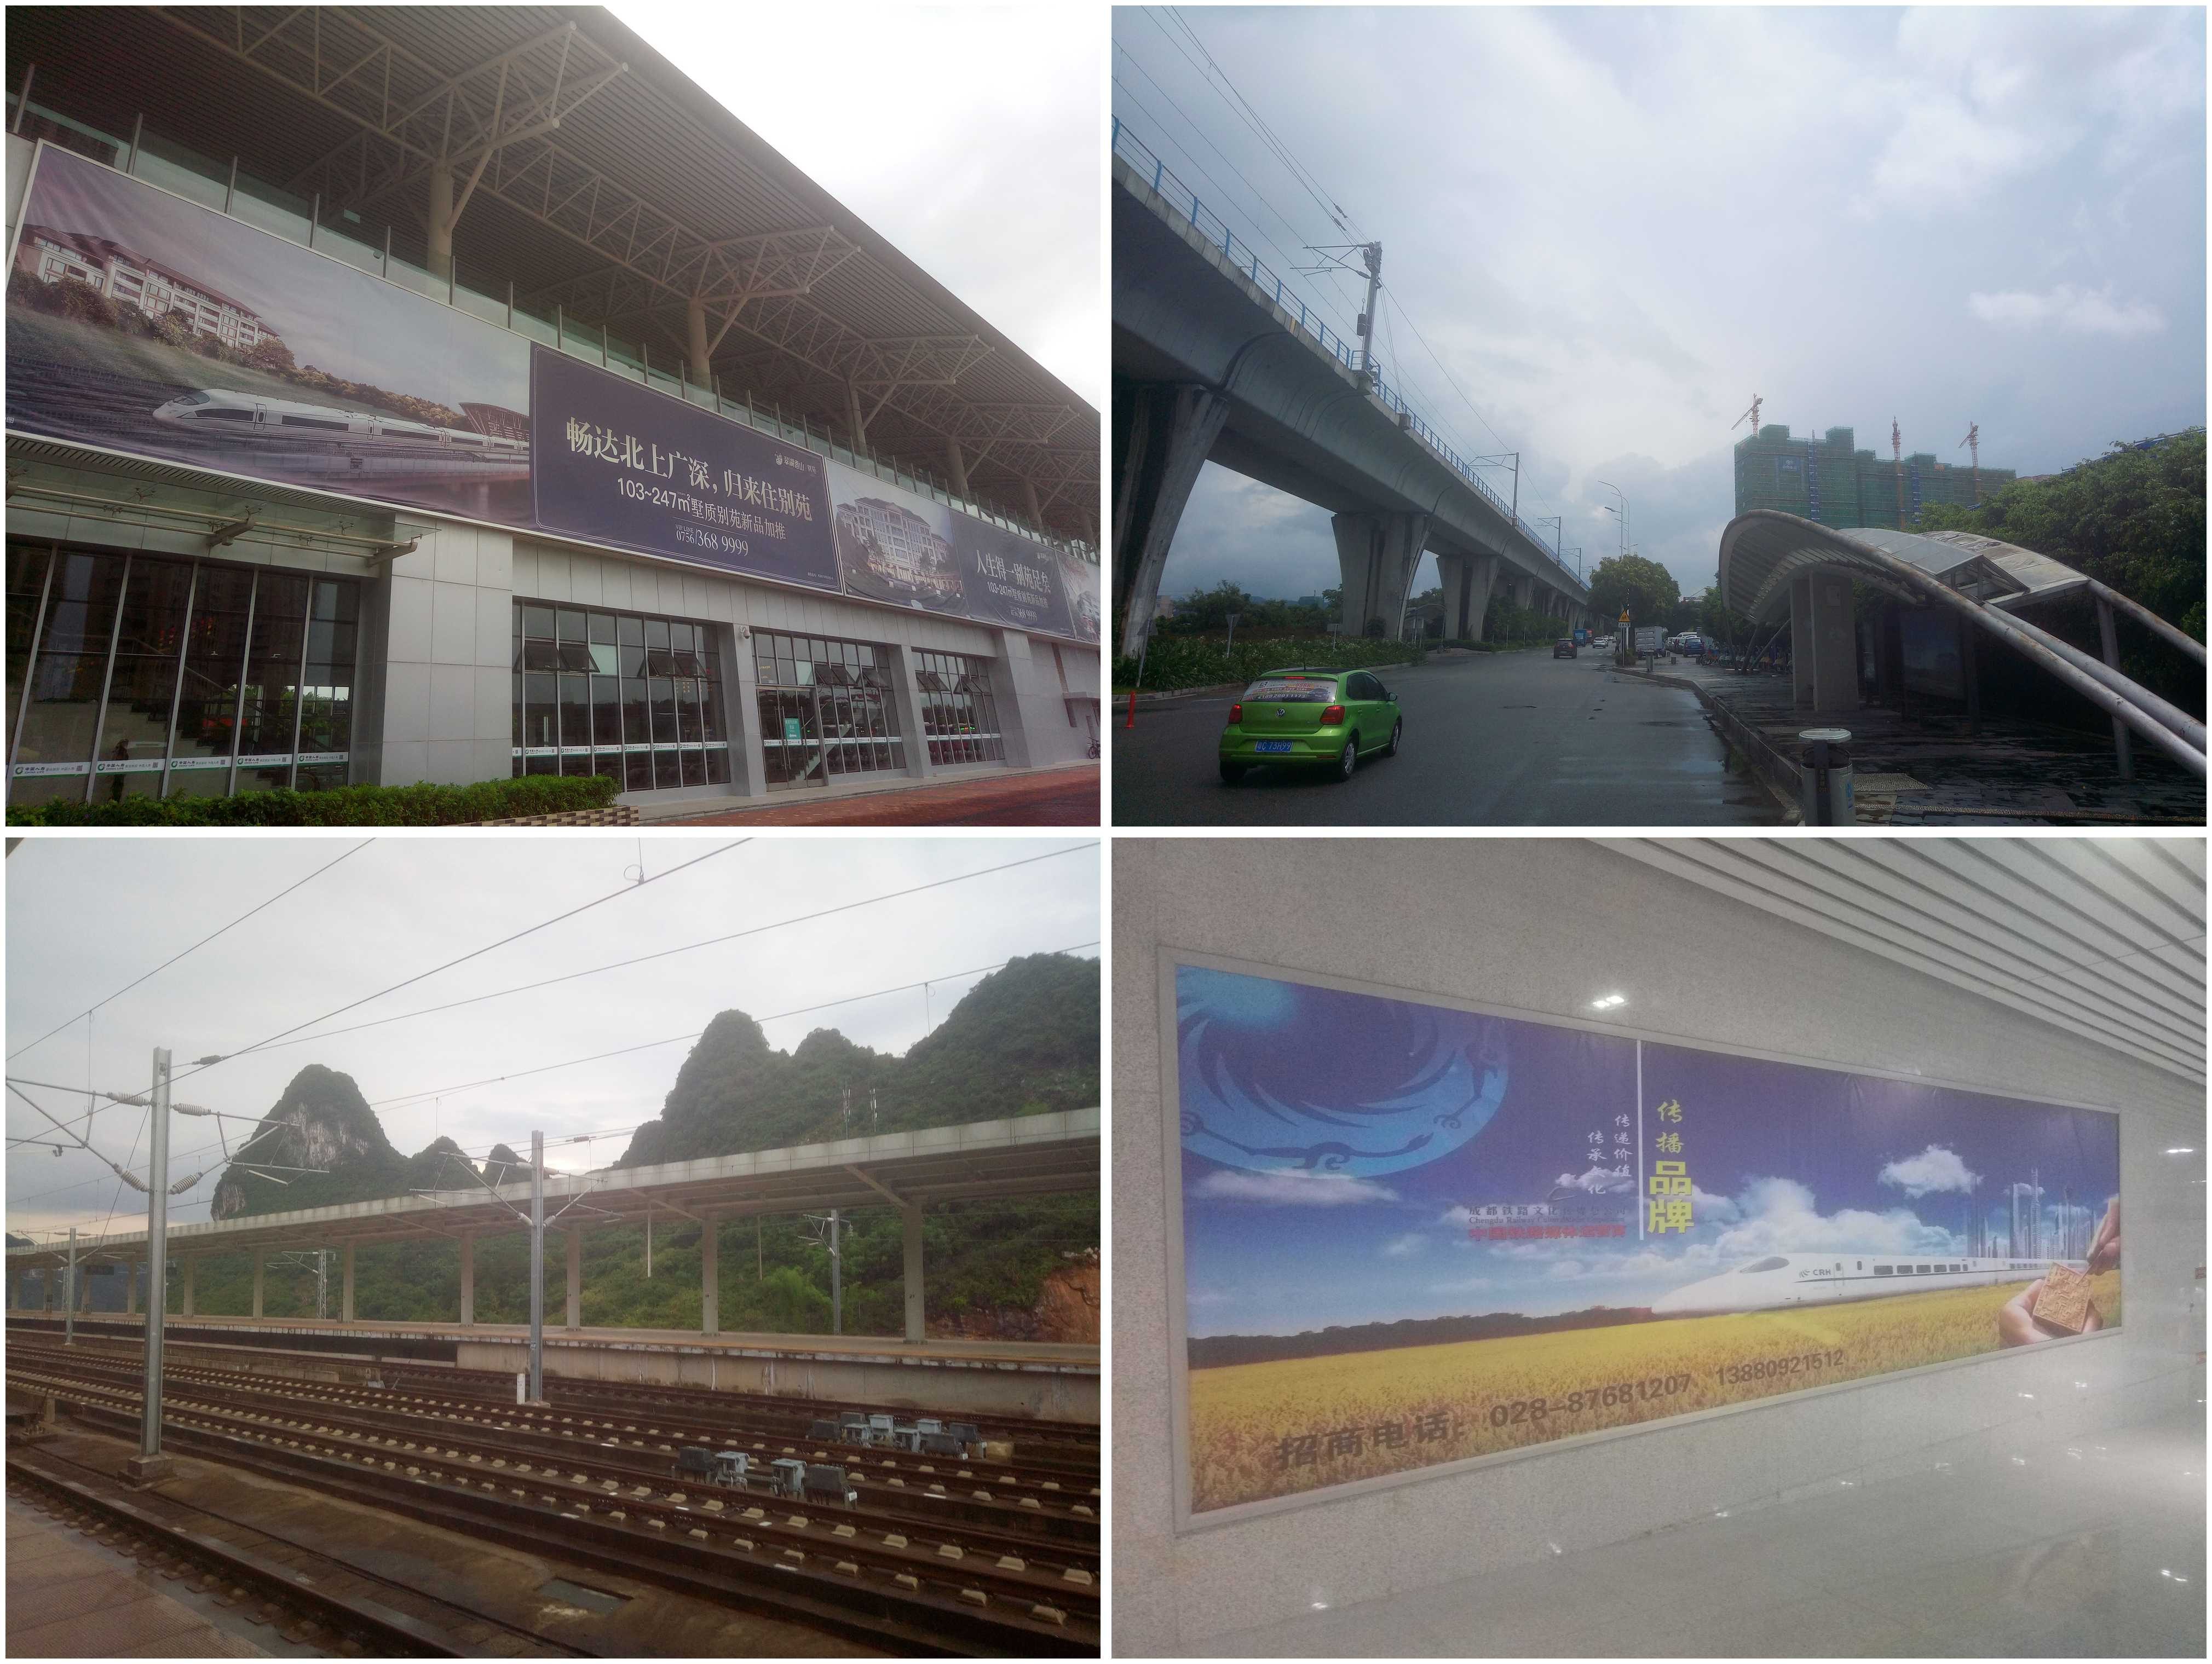
\includegraphics[width=\linewidth]{figures/1-3-1-fig-qualitative-hsr}
	\caption{\textbf{Local manifestations of the mutations induced by the new high speed network.} \textit{(Top Left)} High speed station of Tangjia, in Zhuhai city. The monumental advertisement for a real estate operation praises the merits of the proximity to the network, which is also used as an argument for higher prices; \textit{(Top Right)} High speed line in Zhuhai, deserted bus stop and real estate project being realized in a difficultly accessible area: this urban fringe is in direct contact with the rural environment on the other side of the line, and eccentric from the city; \textit{(Bottom Left)} Yangshuo station on the Guangzhou-Guiyang line, which principal function is the development of this touristic destination which bases most of its economy on that field; \textit{(Bottom Right)} Advertisement for high speed in Sichuan, at the station of the international Chengdu airport on the line to Leshan and Emeishan. The train departs from the futurist city to fly over the countryside, recalling the tunnel effect of territories telescoped by high speed.\label{fig:qualitative:hsr}}
\end{figure}
%%%%%%%%%%%%%


Finally, it is important to remark the network development answers simultaneously to different types of territorial contexts. Branches of the new high speed network with a short range, such as the line Guangzhou-Zhuhai, can be seen as being at the intermediary between a long range service and a proximity regional transport, depending on the modularity of serving patterns. This line is thus placed within long range urban interactions (the service Zhuhai-Guiyang being for example ensured) and within interactions in the mega-city region, most of the service being trains to Guangzhou. To this can be added the classical train network which keeps a certain role in territorial interactions: some connections require the use of both networks and of urban transportation, such as the link between Zhuhai and Hong-Kong, experimented through terrestrial transportation modes only. Indeed, following the Hato Typhoon on 23/08/2017, maritime links with the center of Hong-Kong and the international airport has been interrupted for a significant part of the delta, and has been reopened for Zhuhai in the beginning of November 2017 only, inspiring a fieldwork trip using terrestrial public transportation.


\subsection{Implementing TOD: contrasted illustrations}

The simultaneous development of the transportation network and the urban environment can be directly observed on the field. The local urban network and real estate development operations are planned closely with the new train network: the Zhuhai tramway, for which a single line is open at the current time and still being tested, is thought to participate in a TOD approach\footnote{See preliminary works of planning consulting, such as for example \url{https://wenku.baidu.com/view/b1526461ff00bed5b8f31d01.html} for the context of the new Xiaozhen district, in the West of Xiangzhou.} to urban development which aims at favoring the use of public transportation and a city with less cars, such as wanted for example by the Planning Committee of the \emph{High-Tech Zone} in charge of the development around Zhuhai North station. The observation of the surroundings of Tangjia station, also built in the same spirit, reveals a certain atmosphere of desertion and an unpractical organisation can lead to questioning the efficacy of the approach. This also suggests a certain self-fulfilling nature of the project, as suggested by advertisements for new real estate for sale, insisting on the importance of the presence of the railway line. A full narrative encouraging local actors and individuals to be involved around TOD seems to be used by different actors of development.

Other fieldwork observations, such as in the \emph{New Territories} in Hong-Kong, witness of an efficient TOD which fulfils its objective, with a complementarity between heavy rail and local light tramway, and also a high urban density around stations. These observations recall the complexity of urban trajectories coupled to the development of the network, and that we must remain cautious before drawing any general conclusion from particular cases. We summarize in Fig.~\ref{fig:qualitative:schema} the comparison between the two TOD cases detailed above, as synthetic schemes of urban structures of each area. In Hong-Kong, urban areas have been conjointly planned with the MTR line (heavy transport) and the multiple light tramway lines~\cite{hui2005study}. The infrastructure of light rail and the organisation of missions allow to rapidly connect with the closest station, distributing a highly uniform accessibility for all districts of the territory. On the contrary in Zhuhai, the village of Tangjia is old, even anterior to the rest of Zhuhai, and has developed without any particular articulation with transportation infrastructures. The location of the tramway, which just opened, completes the trajectory of the new railway line, with an objective of reorganizing the North of Zhuhai, and in particular the High-tech Zone which extends from the North railway station (Zhuhai Bei) to Tangjia. Currently, the urban organisation is strongly imprinted with this unsynchronized development, since public transportation accessibility is still relatively low, bus lines being subject to an increasing congestion due to the strong increase in the number of cars. Furthermore, the exploitation of the tramway has been difficult, since the technology used with a third rail in the ground has been imported from Europe and had never been tested in such humidity conditions\footnote{Source: personal communication with \noun{Yinghao Li}, July 2017.}, what lead to a questioning of the network plan in its entirety. 

This fieldwork example thus shows us that (i) under the same designation very different processes exist, and are extremely dependant to geographical, political and economical particularities; and that (ii) the development of a territory which is functional in terms of accessibility necessitates a fine articulation which seems to be the outcome of an integrated planning approach on the long time.

%%%%%%%%%%%%%
\begin{figure}
	%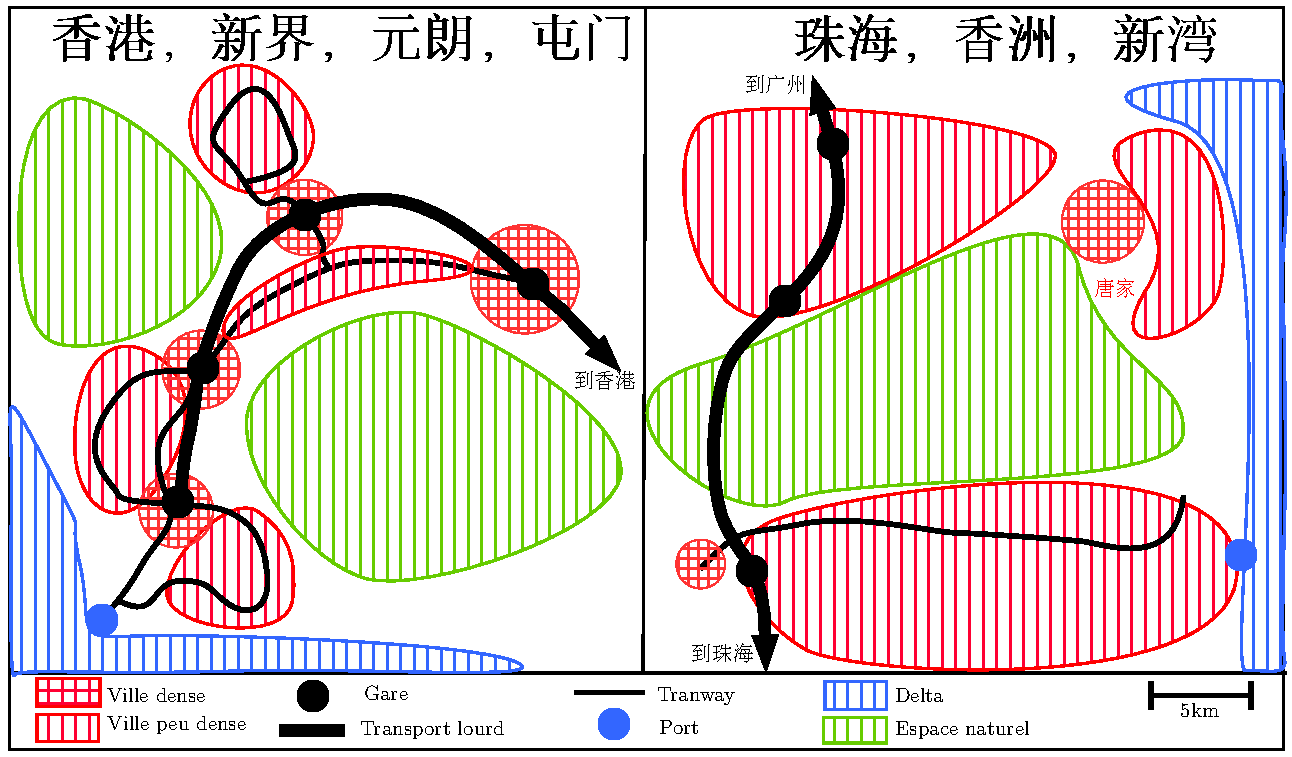
\includegraphics[width=\linewidth]{Figures/Qualitative/tod_fr}
	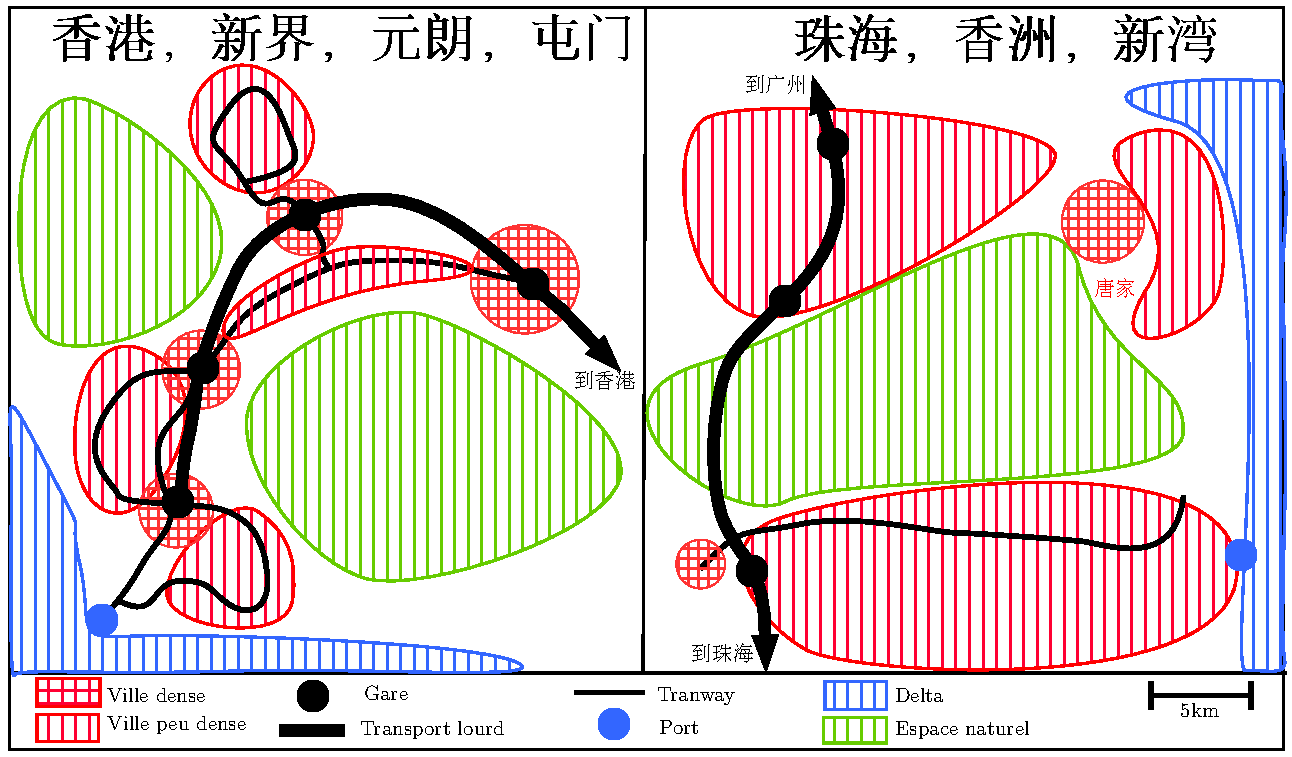
\includegraphics[width=\linewidth]{figures/1-3-1-fig-qualitative-schema.pdf}
	\caption{\textbf{Comparative analysis of two implementations of TOD in PRD.} At a comparable scale, we synthesize the urban configuration of Yuenlong}
	% (\cn{元朗}) and Tuenmun (\cn{屯门}), Hong-Kong New Territories (\cn{香港,新界}), on the left, and of Xinwan, Xiangzhou, Zhuhai (\cn{珠海,香洲,新湾}), on the right, which contains the Zhuhai High-tech zone in its nothern part in particular. The configurations illustrate different dynamics of articulation, and shifted construction temporalities, unveiling thus different realities under the notion of TOD. A first interpretation would be that it is effective if the trajectory of the full territorial system (urban development and transportation network) is modified early in its genesis, whereas a system with a higher level of maturity will have more inertia. \textit{Trans. : } \cn{到香港} - towards Hong-Kong ; \cn{到广州} - towards Guangzhou ; \cn{到珠海} - towards Zhuhai.\label{fig:qualitative:schema}}
\end{figure}
%%%%%%%%%%%%%%

% \subsection{An experiment in floating observation} -> ?



%%%%%%%%%%%%%%%%%%%%
\section{Evolution of accessibility landscapes}

% TODO publish R packages (to be quoted)


% list of cities with urban transit
%. https://en.wikipedia.org/wiki/Urban_rail_transit_in_China
%. => only main for now, but with opening dates ?

% baidu via https://github.com/hotosm/oam-qgis-plugin ?
% OSM + Baidu




%%%%%%%%%%%%%%%%%%%%
\section{Discussion}





%%%%%%%%%%%%%%%%%%%%
\section*{Conclusion}





\section*{Acknowledgements}

% acknowledge Medium project and Chinese partners





%%%%%%%%%%%%%%%%%%%%
%% Biblio
%%%%%%%%%%%%%%%%%%%%


\bibliographystyle{apalike}
\bibliography{biblio}







\end{document}
